%!TEX root = paper.tex
%related.tex

\section{Related work}
\label{sec:related}

\subsection{Imbalances of Power}
This work falls within a line of research that investigates imbalances of power between citizens and institutions, such as governments or corporations. In~\cite{laskowskigovernment}, we investigated the issue of government surveillance.  Our main takeaway was that increased surveillance technology increases incentives for abuse. In  \cite{johnsoncaviar}, we considered the welfare of consumers as a result of corporate exchanges of personal data.
We found that when consumers are myopic, firms benefit greatly, but consumer surplus is also reduced. When we assume consumers are strategic, a more complex picture emerges. Consumers are better off in this case, but firms fare worse.  Given that firms actually do in fact share consumer data in ways quite similar to our model, consumers cannot be acting strategically.  One might wonder, if a market for consumer data only exists when consumers are non-strategic, is the market exploiting consumers?  This work follows this line of investigation on power imbalances by considering the plight of minority groups targeted by unjust laws.

\subsection{Polarization}
Most voters in the United States have been and remain overwhelmingly moderate in their policy positions\cite{layman2006party}. Nevertheless, the United States have passed many laws that are extremely divisive.  Federal laws are passed by the United States congress, which has become increasingly polarized over the last 40 years.
\begin{figure}[htbp]
\begin{center}
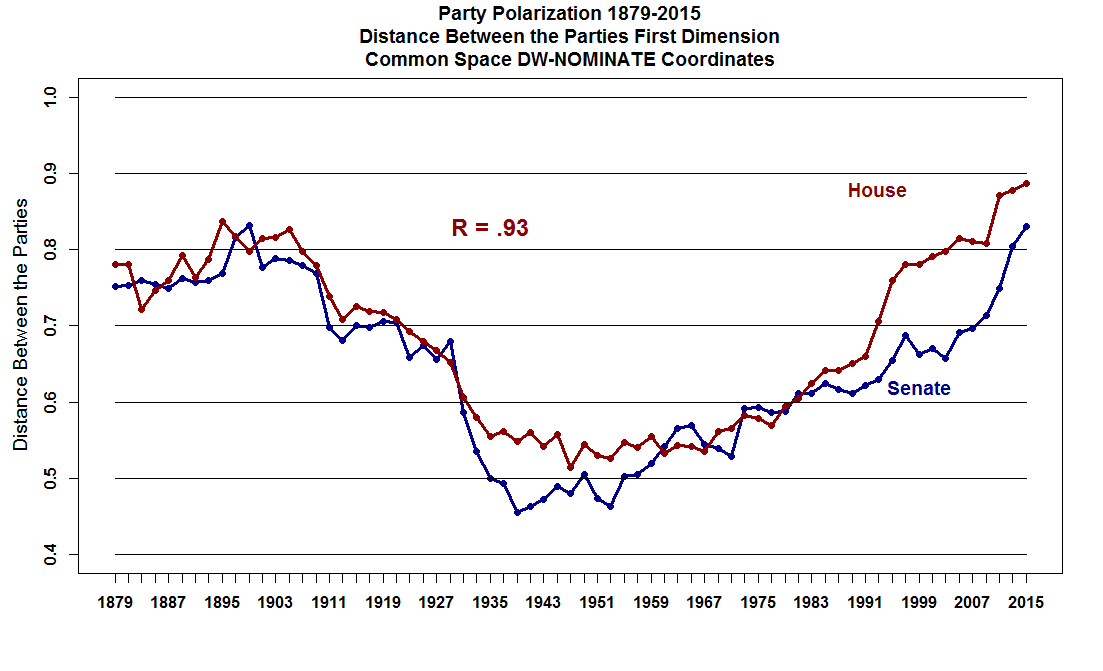
\includegraphics[width=0.4\textwidth]{figs/polar_house_and_senate_46-115_july_11}
\caption{{\bf Polarization Trends in the US Congress}}
\label{fig:uscongress}
\end{center}
\end{figure}

Researchers have posited a number of reasons for this phenomenon, ranging from a polarized electorate, to southern realignment, to gerrymandering, to the evolution of modern primary elections, to economic inequality, to money in politics, to the media environment, or to congress-based factors such as congressional rule changes, majority party agenda control, party pressures, teamsmanship, and a breakdown of bipartisan norms.  All of these are discussed in  \cite{poole1984polarization}

\begin{figure}[htbp]
\begin{center}
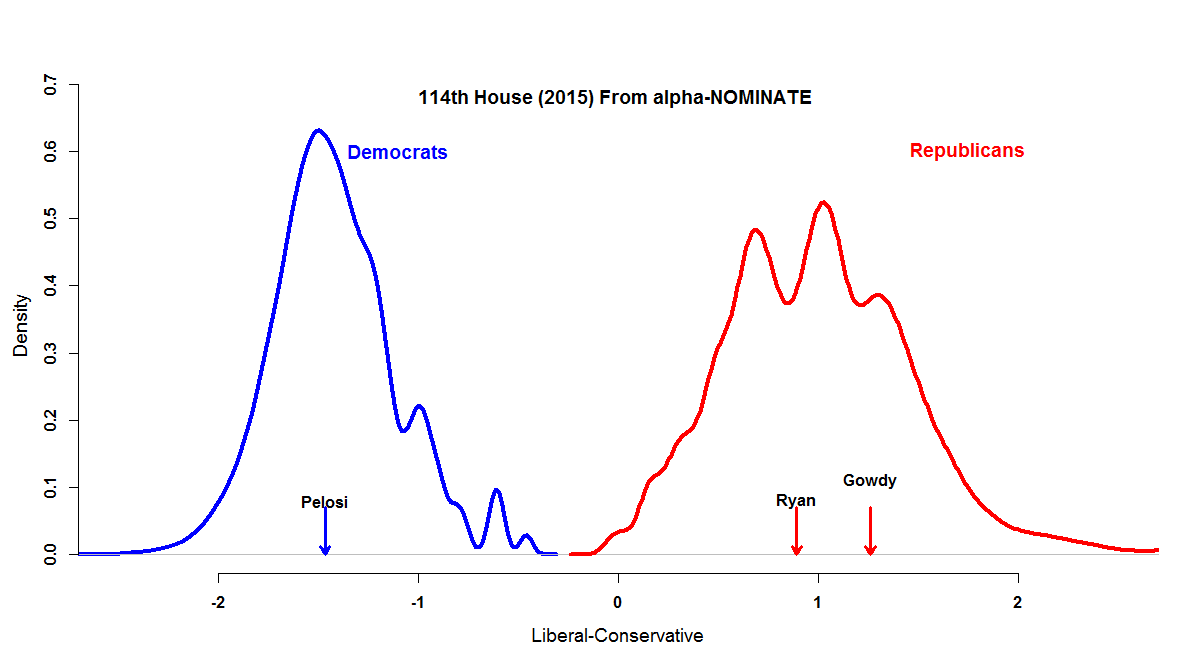
\includegraphics[width=0.4\textwidth]{figs/alpha_House_114_Histogram_8_January_2016}
\caption{{\bf default}}
\label{default}
\end{center}
\end{figure}



\subsection{Privacy}

Privacy on the ground. Hard to find citation in bibtex. Can cite a related journal article instead?

Journal article on polariztion \cite{poole1984polarization}

Book on Authoritarianism \cite{hetherington2009authoritarianism}


Causes and consequences of polarization \cite{barber2015causes}

noisy signals example is informational cascades, people receive a noisy signal and rely on friends and colleagues to distill the essential parts
noisy information signal combined with bayesian updating. 



The notion that people exhibit herding behaviour in predictable circumstances has been around for decades. \cite{shiller1995conversation}

\benjamin{this is plagiarized, must rewrite substantially}
The adoption rate of drought-resistant hybrid seed corn during the Great Depression and Dust Bowl was slow despite its significant improvement over the previously available seed corn. Researchers at Iowa State University were interested in understanding the public's hesitation to the adoption of this significantly improved technology. After conducting 259 interviews with farmers \cite{carboneau2005using} it was observed that the slow rate of adoption was due to how the farmers valued the opinion of their friends and neighbors instead of the word of a salesman. See \cite{beal1957diffusion} for the original report.


\cite{bikhchandani1992theory}
``An information cascade occurs when it is optimal for an individual, having observed the actions of those ahead of him, to follow the begvior of the preceeding individual without regard to his own information."



McCarty, Poole, and Rosenthal (2006) demonstrated a close correlation between economic
inequality and polarization in the United States


polarized electorate, southern realignment, Gerrymandering, primary elections, economic inequality, money in politics, media environment, congress-based factors such as congressional rule changes, majority party agenda control, party pressures, teamsmanship, breakdown of bipartisan norms.  All of these are discussed in  \cite{poole1984polarization}